\documentclass[../Notes.tex]{subfiles}
\usepackage{../Style/Diagrams}
\usepackage{../Style/Master}
\usepackage{../Style/boxes}
\usepackage{../Style/DefNoteFact}
\usepackage{../Style/QnsProof}
\usepackage{../Style/Thms}
\usepackage{../Style/Env}
\usepackage{../Style/NewCommands}
\begin{document}
\chapter{Chi-Squared \(\chi^2\) Tests}
\begin{definition}{}{}
  A random variable \(X\) is said to follow a \(\chi^2\)-distribution, with degree of freedom \(\nu\), iff its probability density function is given by
  \[f(x)=\begin{cases}
    \frac{1}{2^{\nu/2}\Gamma(\nu/2)}x^{(\nu/2)-1}e^{-x/2} &\text{if \(x>0\)},\\
    0 &\text{otherwise}.
  \end{cases}\]
\end{definition}
\begin{stbox}{General Information}
  \begin{itemize}
    \item Properties of chi-squared distributions.
    \begin{itemize}
      \item \(\E(X)=v\) and \(\Var(X)=2\nu\).
      % , and the mode of \(X\) is \(\max\{k-2,0\}\).
      \item The \(\chi_{(\nu)}^2\) distribution tends to a normal distribution as \(\nu\to\infty\).
      \item Suppose \(Z_i\sim\Normal(0,1)\) are independent. Then, \(Z_1^2+\dots+Z_n^2\sim\chi^2_{(n)}\).
      \item If \(X\sim\chi_{(\nu)}^2\) and \(Y\sim\chi_{(\upsilon)}^2\), then \(X+Y\sim\chi_{(\nu+\upsilon)}^2\).
      \item 
    \end{itemize}
  \end{itemize}
\end{stbox}
% Insert figure
\begin{stbox}{}
  \begin{itemize}
    \item A goodness-of-fit test.
    \begin{enumerate}
      \item Let [\(X\) in context] and \(\mu\) be the population mean.
      \item 
      \begin{tabular}{|ll|}
        \hline
        Test & \(H_0\colon\text{[\(X\) follows the distribution in context]}\)\\
        against &\(H_1\colon\text{[\(X\) does not follows the distribution in context]}\)\\
        \multicolumn{2}{|l|}{at the \(100\alpha\%\) significance level.}\\
        \hline
      \end{tabular}
      \item Under \(H_0\), the test statistic
      \[T=\frac{\widebar{X}-\mu}{s/\sqrt{n}}\sim t(n-1).\]
      \item Continue as per usual, calculating the critical region or the \(p\)-value.
    \end{enumerate}
  \end{itemize}
\end{stbox}
\begin{note}
  If \(X\) follows a \emph{discrete} normal distribution, we must state it out in words. We cannot say \(X\sim\Normal(\mu,\sigma^2)\) as this would denote that \(X\) is a \emph{continuous} random variable. 
\end{note}

\chapter{Correlation and Linear Regression}
\begin{note}
  A good scatter diagram should follow the guidelines below.
  \begin{itemize}
    \item The relative position of each point on the scatter diagram should be clearly shown.
    \item The range of values for the set of data should be clearly shown by marking out the extreme \(x\) and \(y\) values on the corresponding axis.
    \item The axes should be labeled clearly with the variables.
  \end{itemize}
\end{note}
\begin{stbox}{General Information}
  \begin{itemize}
    \item The Product Moment Correlation Coefficient is a measure of the linear correlation between two variables. It is defined by
    \[r=\frac{\sum{(x-\bar{x})(y-\bar{y})}}{\sqrt{\sum{(x-\bar{x})^2}\sum{(y-\bar{y})^2}}}=\frac{\sum{xy}-\dfrac{\sum{x}\sum{y}}{n}}{\sqrt{\left[\sum{x^2}-\dfrac{\left(\sum{x}\right)^2}{n}\right]\left[\sum{y^2}-\dfrac{\left(\sum{y}\right)^2}{n}\right]}},\]
    which takes on a value from 0 to 1.
    \item When \(r=0\), there is no linear relationship. But, a nonlinear relationship may be present. Additionally, the regression lines are perpendicular.
    \item The closer the value of \(r\) is to 1 (or -1), the stronger the positive (or negative) linear correlation. Furthermore, the regression lines coincide.
    \begin{center}
      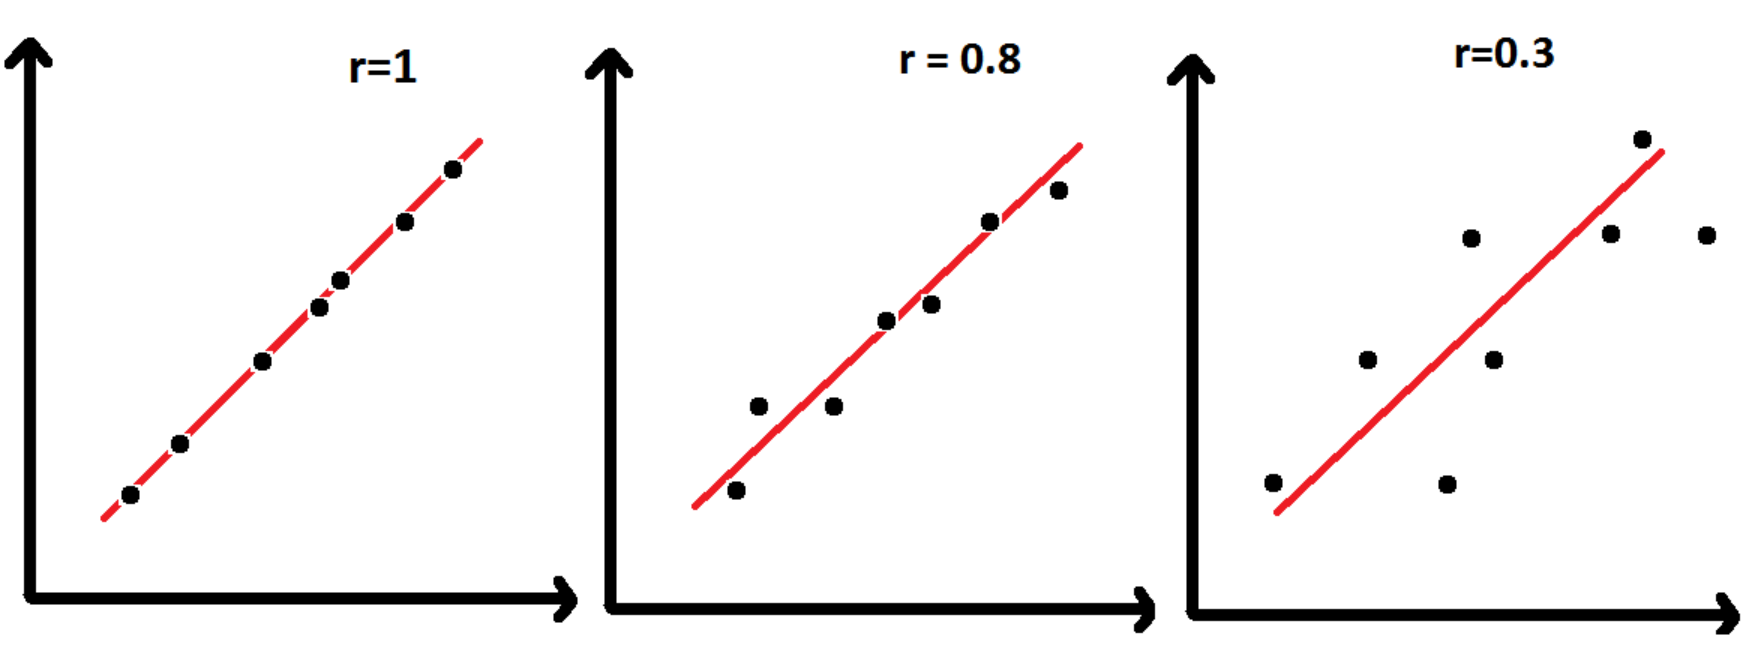
\includegraphics[scale=0.3]{../images/Product Moment Correlation Coefficient 1.png}
      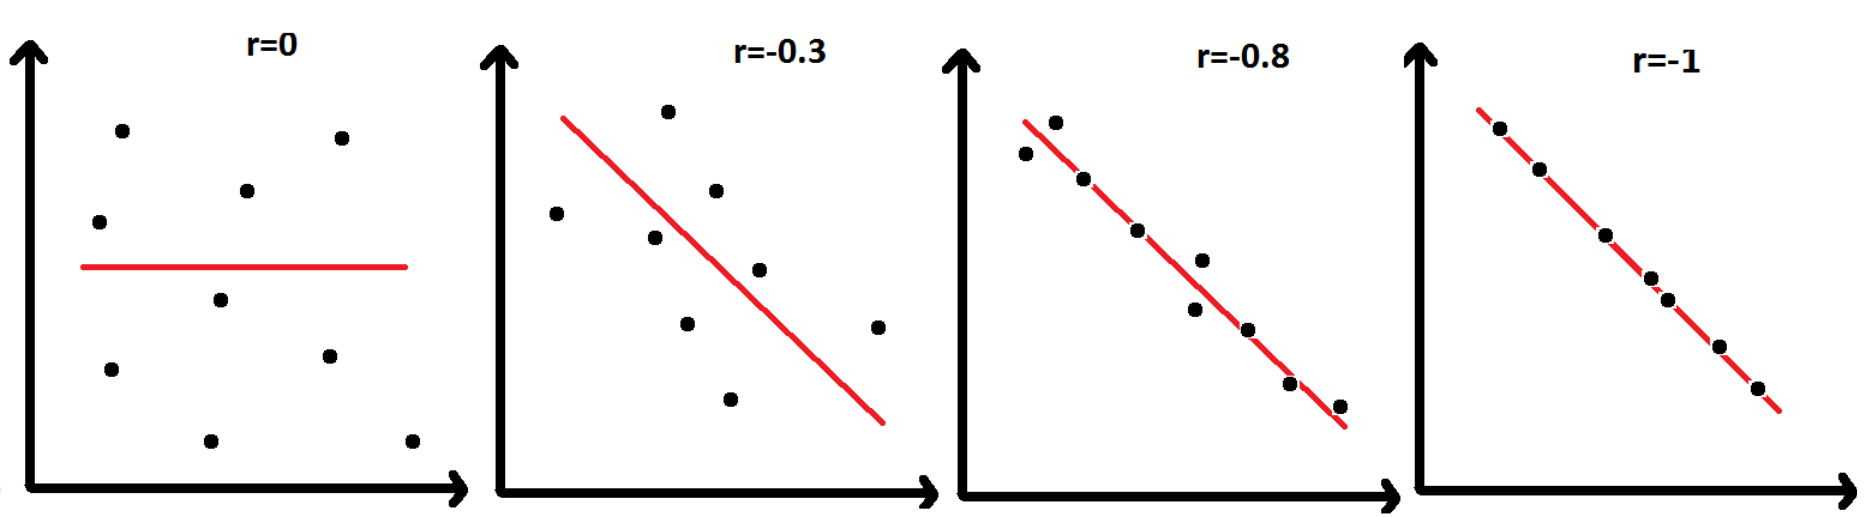
\includegraphics[scale=0.4]{../images/Product Moment Correlation Coefficient 2.png}
    \end{center}
    \item The regression line of \(y\) on \(x\) minimises the sum of squares deviation (error) in the \(y\)-direction. (i.e. we are assuming \(x\) is the independent variable whose values are known exactly.) It is given by
    \[y=\bar{y}+b(x-\bar{x}),\qquad\text{where}\qquad b=\frac{\sum{(x-\bar{x})(y-\bar{y})}}{\sum{(x-\bar{x})^2}}=\frac{\sum{xy}-\dfrac{\sum{x}\sum{y}}{n}}{\sum{x^2}-\dfrac{\left(\sum{x}\right)^2}{n}}.\] 
    \item The point \((\bar{x},\bar{y})\) always lies on both the regression lines of \(y\) on \(x\), and \(x\) on \(y\).
    \item Say we are given the value of one variable, and asked to approximate the the value of the other variable. Then, we should always use the line of the \emph{dependent} variable on the \emph{independent}.
    \item Estimations should not be taken for data outside the range of the sample provided, even if the value of \(r\) is close to 1.
  \end{itemize}
\end{stbox}
\end{document}